%File: anonymous-submission-latex-2024.tex
\documentclass[letterpaper]{article} % DO NOT CHANGE THIS
\usepackage[submission]{aaai24}  % DO NOT CHANGE THIS
\usepackage{times}  % DO NOT CHANGE THIS
\usepackage{helvet}  % DO NOT CHANGE THIS
\usepackage{courier}  % DO NOT CHANGE THIS
\usepackage[hyphens]{url}  % DO NOT CHANGE THIS
\usepackage{graphicx} % DO NOT CHANGE THIS
\urlstyle{rm} % DO NOT CHANGE THIS
\def\UrlFont{\rm}  % DO NOT CHANGE THIS
\usepackage{natbib}  % DO NOT CHANGE THIS AND DO NOT ADD ANY OPTIONS TO IT
\usepackage{caption} % DO NOT CHANGE THIS AND DO NOT ADD ANY OPTIONS TO IT
\frenchspacing  % DO NOT CHANGE THIS
\setlength{\pdfpagewidth}{8.5in} % DO NOT CHANGE THIS
\setlength{\pdfpageheight}{11in} % DO NOT CHANGE THIS
%
% These are recommended to typeset algorithms but not required. See the subsubsection on algorithms. Remove them if you don't have algorithms in your paper.
\usepackage{algorithm}
% \usepackage{algorithmic}

%
% These are are recommended to typeset listings but not required. See the subsubsection on listing. Remove this block if you don't have listings in your paper.
% \usepackage{newfloat}
% \usepackage{listings}
% \DeclareCaptionStyle{ruled}{labelfont=normalfont,labelsep=colon,strut=off} % DO NOT CHANGE THIS
% \lstset{%
% 	basicstyle={\footnotesize\ttfamily},% footnotesize acceptable for monospace
% 	numbers=left,numberstyle=\footnotesize,xleftmargin=2em,% show line numbers, remove this entire line if you don't want the numbers.
% 	aboveskip=0pt,belowskip=0pt,%
% 	showstringspaces=false,tabsize=2,breaklines=true}
% \floatstyle{ruled}
% \newfloat{listing}{tb}{lst}{}
% \floatname{listing}{Listing}
%
% Keep the \pdfinfo as shown here. There's no need
% for you to add the /Title and /Author tags.
\pdfinfo{
/TemplateVersion (2024.1)
}

\usepackage{amsfonts}       % blackboard math symbols
\usepackage{amsmath}
\usepackage{amsthm}
\usepackage{caption}
\usepackage{graphicx}
\usepackage{algpseudocode}
\usepackage{import}
\usepackage{booktabs}
\usepackage{longtable}
\usepackage{array}
\usepackage{multirow}


% Numbered Environments:
\newtheorem{definition}{Definition}[section]
\newtheorem{question}{Research Question}[section]

% Bibliography
% \bibliographystyle{unsrtnat}
% \setcitestyle{numbers,square,comma}

% Algorithm
\renewcommand{\algorithmicrequire}{\textbf{Input:}}
\renewcommand{\algorithmicensure}{\textbf{Output:}}

% DISALLOWED PACKAGES
% \usepackage{authblk} -- This package is specifically forbidden
% \usepackage{balance} -- This package is specifically forbidden
% \usepackage{color (if used in text)
% \usepackage{CJK} -- This package is specifically forbidden
% \usepackage{float} -- This package is specifically forbidden
% \usepackage{flushend} -- This package is specifically forbidden
% \usepackage{fontenc} -- This package is specifically forbidden
% \usepackage{fullpage} -- This package is specifically forbidden
% \usepackage{geometry} -- This package is specifically forbidden
% \usepackage{grffile} -- This package is specifically forbidden
% \usepackage{hyperref} -- This package is specifically forbidden
% \usepackage{navigator} -- This package is specifically forbidden
% (or any other package that embeds links such as navigator or hyperref)
% \indentfirst} -- This package is specifically forbidden
% \layout} -- This package is specifically forbidden
% \multicol} -- This package is specifically forbidden
% \nameref} -- This package is specifically forbidden
% \usepackage{savetrees} -- This package is specifically forbidden
% \usepackage{setspace} -- This package is specifically forbidden
% \usepackage{stfloats} -- This package is specifically forbidden
% \usepackage{tabu} -- This package is specifically forbidden
% \usepackage{titlesec} -- This package is specifically forbidden
% \usepackage{tocbibind} -- This package is specifically forbidden
% \usepackage{ulem} -- This package is specifically forbidden
% \usepackage{wrapfig} -- This package is specifically forbidden
% DISALLOWED COMMANDS
% \nocopyright -- Your paper will not be published if you use this command
% \addtolength -- This command may not be used
% \balance -- This command may not be used
% \baselinestretch -- Your paper will not be published if you use this command
% \clearpage -- No page breaks of any kind may be used for the final version of your paper
% \columnsep -- This command may not be used
% \newpage -- No page breaks of any kind may be used for the final version of your paper
% \pagebreak -- No page breaks of any kind may be used for the final version of your paperr
% \pagestyle -- This command may not be used
% \tiny -- This is not an acceptable font size.
% \vspace{- -- No negative value may be used in proximity of a caption, figure, table, section, subsection, subsubsection, or reference
% \vskip{- -- No negative value may be used to alter spacing above or below a caption, figure, table, section, subsection, subsubsection, or reference

\setcounter{secnumdepth}{0} %May be changed to 1 or 2 if section numbers are desired.

% The file aaai24.sty is the style file for AAAI Press
% proceedings, working notes, and technical reports.
%

% Title

% Your title must be in mixed case, not sentence case.
% That means all verbs (including short verbs like be, is, using,and go),
% nouns, adverbs, adjectives should be capitalized, including both words in hyphenated terms, while
% articles, conjunctions, and prepositions are lower case unless they
% directly follow a colon or long dash
\title{AAAI Press Anonymous Submission\\Instructions for Authors Using \LaTeX{}}
\author{
    %Authors
    % All authors must be in the same font size and format.
    Written by AAAI Press Staff\textsuperscript{\rm 1}\thanks{With help from the AAAI Publications Committee.}\\
    AAAI Style Contributions by Pater Patel Schneider,
    Sunil Issar,\\
    J. Scott Penberthy,
    George Ferguson,
    Hans Guesgen,
    Francisco Cruz\equalcontrib,
    Marc Pujol-Gonzalez\equalcontrib
}
\affiliations{
    %Afiliations
    \textsuperscript{\rm 1}Association for the Advancement of Artificial Intelligence\\
    % If you have multiple authors and multiple affiliations
    % use superscripts in text and roman font to identify them.
    % For example,

    % Sunil Issar\textsuperscript{\rm 2},
    % J. Scott Penberthy\textsuperscript{\rm 3},
    % George Ferguson\textsuperscript{\rm 4},
    % Hans Guesgen\textsuperscript{\rm 5}
    % Note that the comma should be placed after the superscript

    1900 Embarcadero Road, Suite 101\\
    Palo Alto, California 94303-3310 USA\\
    % email address must be in roman text type, not monospace or sans serif
    proceedings-questions@aaai.org
%
% See more examples next
}

%Example, Single Author, ->> remove \iffalse,\fi and place them surrounding AAAI title to use it
\iffalse
\title{My Publication Title --- Single Author}
\author {
    Author Name
}
\affiliations{
    Affiliation\\
    Affiliation Line 2\\
    name@example.com
}
\fi

\iffalse
%Example, Multiple Authors, ->> remove \iffalse,\fi and place them surrounding AAAI title to use it
\title{My Publication Title --- Multiple Authors}
\author {
    % Authors
    First Author Name\textsuperscript{\rm 1},
    Second Author Name\textsuperscript{\rm 2},
    Third Author Name\textsuperscript{\rm 1}
}
\affiliations {
    % Affiliations
    \textsuperscript{\rm 1}Affiliation 1\\
    \textsuperscript{\rm 2}Affiliation 2\\
    firstAuthor@affiliation1.com, secondAuthor@affilation2.com, thirdAuthor@affiliation1.com
}
\fi


% REMOVE THIS: bibentry
% This is only needed to show inline citations in the guidelines document. You should not need it and can safely delete it.
\usepackage{bibentry}
% END REMOVE bibentry

\begin{document}

\maketitle

  \begin{abstract}
    Counterfactual Explanations offer an intuitive and straightforward way to explain black-box models and offer Algorithmic Recourse to individuals. To address the need for plausible explanations, existing work has primarily relied on surrogate models to learn how the input data is distributed. This effectively reallocates the task of learning realistic explanations for the data from the model itself to the surrogate. Consequently, the generated explanations may seem plausible to humans but need not necessarily describe the behaviour of the black-box model faithfully. We formalise this notion of faithfulness through the introduction of a tailored evaluation metric and propose a novel algorithmic framework for generating \textbf{E}nergy-\textbf{C}onstrained \textbf{C}onformal \textbf{Co}unterfactuals (ECCCos) that are only as plausible as the model permits. Through extensive empirical studies, we demonstrate that ECCCos reconcile the need for faithfulness and plausibility. In particular, we show that for models with gradient access, it is possible to achieve state-of-the-art performance without the need for surrogate models. To do so, our framework relies solely on properties defining the black-box model itself by leveraging recent advances in Energy-Based Modelling and Conformal Prediction. To our knowledge, this is the first venture in this direction for generating faithful Counterfactual Explanations. Thus, we anticipate that ECCCos can serve as a baseline for future research. We believe that our work opens avenues for researchers and practitioners seeking tools to better distinguish trustworthy from unreliable models.
  \end{abstract}
  
  \section{Introduction}\label{intro}
  
  Counterfactual Explanations (CE) provide a powerful, flexible and intuitive way to not only explain black-box models but also help affected individuals through the means of Algorithmic Recourse. Instead of opening the Black Box, CE works under the premise of strategically perturbing model inputs to understand model behaviour~\citep{wachter2017counterfactual}. Intuitively speaking, we generate explanations in this context by asking what-if questions of the following nature: `Our credit risk model currently predicts that this individual is not credit-worthy. What if they reduced their monthly expenditures by 10\%?'
  
  This is typically implemented by defining a target outcome $\mathbf{y}^+ \in \mathcal{Y}$ for some individual $\mathbf{x} \in \mathcal{X}=\mathbb{R}^D$ described by $D$ attributes, for which the model $M_{\theta}:\mathcal{X}\mapsto\mathcal{Y}$ initially predicts a different outcome: $M_{\theta}(\mathbf{x})\ne \mathbf{y}^+$. Counterfactuals are then searched by minimizing a loss function that compares the predicted model output to the target outcome: $\text{yloss}(M_{\theta}(\mathbf{x}),\mathbf{y}^+)$. Since CE work directly with the black-box model, valid counterfactuals always have full local fidelity by construction where fidelity is defined as the degree to which explanations approximate the predictions of a black-box model~\citep{mothilal2020explaining,molnar2020interpretable}. 
  
  In situations where full fidelity is a requirement, CE offer a more appropriate solution to Explainable Artificial Intelligence (XAI) than other popular approaches like LIME~\citep{ribeiro2016why} and SHAP~\citep{lundberg2017unified}, which involve local surrogate models. But even full fidelity is not a sufficient condition for ensuring that an explanation faithfully describes the behaviour of a model. That is because multiple very distinct explanations can all lead to the same model prediction, especially when dealing with heavily parameterized models like deep neural networks, which are typically underspecified by the data~\citep{wilson2020case}.
  
  In the context of CE, the idea that no two explanations are the same arises almost naturally. A key focus in the literature has therefore been to identify those explanations and algorithmic recourses that are most appropriate based on a myriad of desiderata such as sparsity, actionability and plausibility. In this work, we draw closer attention to model faithfulness rather than fidelity as a desideratum for counterfactuals. Our key contributions are as follows: 
  
  \begin{itemize}
    \item We show that fidelity is an insufficient evaluation metric for counterfactuals (Section~\ref{fidelity}) and propose a definition of faithfulness that gives rise to more suitable metrics (Section~\ref{faithfulness}).
    \item We introduce a novel algorithmic approach for generating Energy-Constrained Conformal Counterfactuals (ECCCos) in Section~\ref{meth}.
    \item We provide extensive empirical evidence demonstrating that ECCCos faithfully explain model behaviour and attain plausibility only when appropriate (Section~\ref{emp}).
  \end{itemize}
  
  To our knowledge, this is the first venture in this direction for generating faithful counterfactuals. Thus, we anticipate that ECCCos can serve as a baseline for future research. We believe that our work opens avenues for researchers and practitioners seeking tools to better distinguish trustworthy from unreliable models.
  
  \section{Background}\label{background}
  
  While CE can also be generated for arbitrary regression models~\citep{spooner2021counterfactual}, existing work has primarily focused on classification problems. Let $\mathcal{Y}=(0,1)^K$ denote the one-hot-encoded output domain with $K$ classes. Then most counterfactual generators rely on gradient descent to optimize different flavours of the following counterfactual search objective:
  
  \begin{equation} \label{eq:general}
  \begin{aligned}
  \mathbf{Z}^\prime &= \arg \min_{\mathbf{Z}^\prime \in \mathcal{Z}^L} \left\{  {\text{yloss}(M_{\theta}(f(\mathbf{Z}^\prime)),\mathbf{y}^+)}+ \lambda {\text{cost}(f(\mathbf{Z}^\prime)) }  \right\} 
  \end{aligned} 
  \end{equation}
  
  Here $\text{yloss}(\cdot)$ denotes the primary loss function, $f(\cdot)$ is a function that maps from the counterfactual state space to the feature space and $\text{cost}(\cdot)$ is either a single penalty or a collection of penalties that are used to impose constraints through regularization. Equation~\ref{eq:general} restates the baseline approach to gradient-based counterfactual search proposed by~\citet{wachter2017counterfactual} in general form as introduced by~\citet{altmeyer2023endogenous}. To explicitly account for the multiplicity of explanations, $\mathbf{Z}^\prime=\{ \mathbf{z}_l\}_L$ denotes an $L$-dimensional array of counterfactual states. 
  
  The baseline approach, which we will simply refer to as \textit{Wachter}, searches a single counterfactual directly in the feature space and penalises its distance to the original factual. In this case, $f(\cdot)$ is simply the identity function and $\mathcal{Z}$ corresponds to the feature space itself. Many derivative works of~\citet{wachter2017counterfactual} have proposed new flavours of Equation~\ref{eq:general}, each of them designed to address specific \textit{desiderata} that counterfactuals ought to meet in order to properly serve both AI practitioners and individuals affected by algorithmic decision-making systems. The list of desiderata includes but is not limited to the following: sparsity, proximity~\citep{wachter2017counterfactual}, actionability~\citep{ustun2019actionable}, diversity~\citep{mothilal2020explaining}, plausibility~\citep{joshi2019realistic,poyiadzi2020face,schut2021generating}, robustness~\citep{upadhyay2021robust,pawelczyk2022probabilistically,altmeyer2023endogenous} and causality~\citep{karimi2021algorithmic}. Different counterfactual generators addressing these needs have been extensively surveyed and evaluated in various studies~\citep{verma2020counterfactual,karimi2020survey,pawelczyk2021carla,artelt2021evaluating,guidotti2022counterfactual}. 
  
  Perhaps unsurprisingly, the different desiderata are often positively correlated. For example, \citet{artelt2021evaluating} find that plausibility typically also leads to improved robustness. Similarly, plausibility has also been connected to causality in the sense that plausible counterfactuals respect causal relationships~\citep{mahajan2020preserving}. Consequently, the plausibility of counterfactuals has been among the primary concerns for researchers. Achieving plausibility is equivalent to ensuring that the generated counterfactuals comply with the true and unobserved data-generating process (DGP). We define plausibility formally in this work as follows:
  
  \begin{definition}[Plausible Counterfactuals]
    \label{def:plausible}
    Let $\mathcal{X}|\mathbf{y}^+= p(\mathbf{x}|\mathbf{y}^+)$ denote the true conditional distribution of samples in the target class $\mathbf{y}^+$. Then for $\mathbf{x}^{\prime}$ to be considered a plausible counterfactual, we need: $\mathbf{x}^{\prime} \sim \mathcal{X}|\mathbf{y}^+$.
  \end{definition}
  
  To generate plausible counterfactuals, we need to be able to quantify the DGP: $\mathcal{X}|\mathbf{y}^+$. One straightforward way to do this is to use surrogate models for the task. \citet{joshi2019realistic}, for example, suggest that instead of searching counterfactuals in the feature space $\mathcal{X}$, we can instead traverse a latent embedding $\mathcal{Z}$ (Equation~\ref{eq:general}) that implicitly codifies the DGP. To learn the latent embedding, they propose using a generative model such as a Variational Autoencoder (VAE). Provided the surrogate model is well-specified, their proposed approach called \textit{REVISE} can yield plausible explanations. Others have proposed similar approaches: \citet{dombrowski2021diffeomorphic} traverse the base space of a normalizing flow to solve Equation~\ref{eq:general}; \citet{poyiadzi2020face} use density estimators ($\hat{p}: \mathcal{X} \mapsto [0,1]$) to constrain the counterfactuals to dense regions in the feature space; and, finally, \citet{karimi2021algorithmic} assume knowledge about the structural causal model that generates the data.
  
  A competing approach towards plausibility that is also closely related to this work instead relies on the black-box model itself. \citet{schut2021generating} show that to meet the plausibility objective we need not explicitly model the input distribution. Pointing to the undesirable engineering overhead induced by surrogate models, they propose that we rely on the implicit minimisation of predictive uncertainty instead. Their proposed methodology, which we will refer to as \textit{Schut}, solves Equation~\ref{eq:general} by greedily applying Jacobian-Based Saliency Map Attacks (JSMA) in the feature space with cross-entropy loss and no penalty at all. The authors demonstrate theoretically and empirically that their approach yields counterfactuals for which the model $M_{\theta}$ predicts the target label $\mathbf{y}^+$ with high confidence. Provided the model is well-specified, these counterfactuals are plausible. This idea hinges on the assumption that the black-box model provides well-calibrated predictive uncertainty estimates.
  
  \section{Why Fidelity is not Enough}\label{fidelity}
  
  As discussed in the introduction, any valid counterfactual also has full fidelity by construction: solutions to Equation~\ref{eq:general} are considered valid as soon as the label predicted by the model matches the target class. So while fidelity always applies, counterfactuals that address the various desiderata introduced above can look vastly different from each other. 
  
  To demonstrate this with an example, we have trained a simple image classifier $M_{\theta}$ on the well-known \textit{MNIST} dataset~\citep{lecun1998mnist}: a Multi-Layer Perceptron (\textit{MLP}) with above 90 percent test accuracy. No measures have been taken to improve the model's adversarial robustness or its capacity for predictive uncertainty quantification. The far left panel of Figure ~\ref{fig:motiv} shows a random sample drawn from the dataset. The underlying classifier correctly predicts the label `nine' for this image. For the given factual image and model, we have used \textit{Wachter}, \textit{Schut} and \textit{REVISE} to generate one counterfactual each in the target class `seven'. The perturbed images are shown next to the factual image from left to right in Figure ~\ref{fig:motiv}. Captions on top of the individual images indicate the generator along with the predicted probability that the image belongs to the target class. In all three cases that probability is above 90 percent and yet the counterfactuals look very different from each other.
  
  \begin{figure}
    \centering
    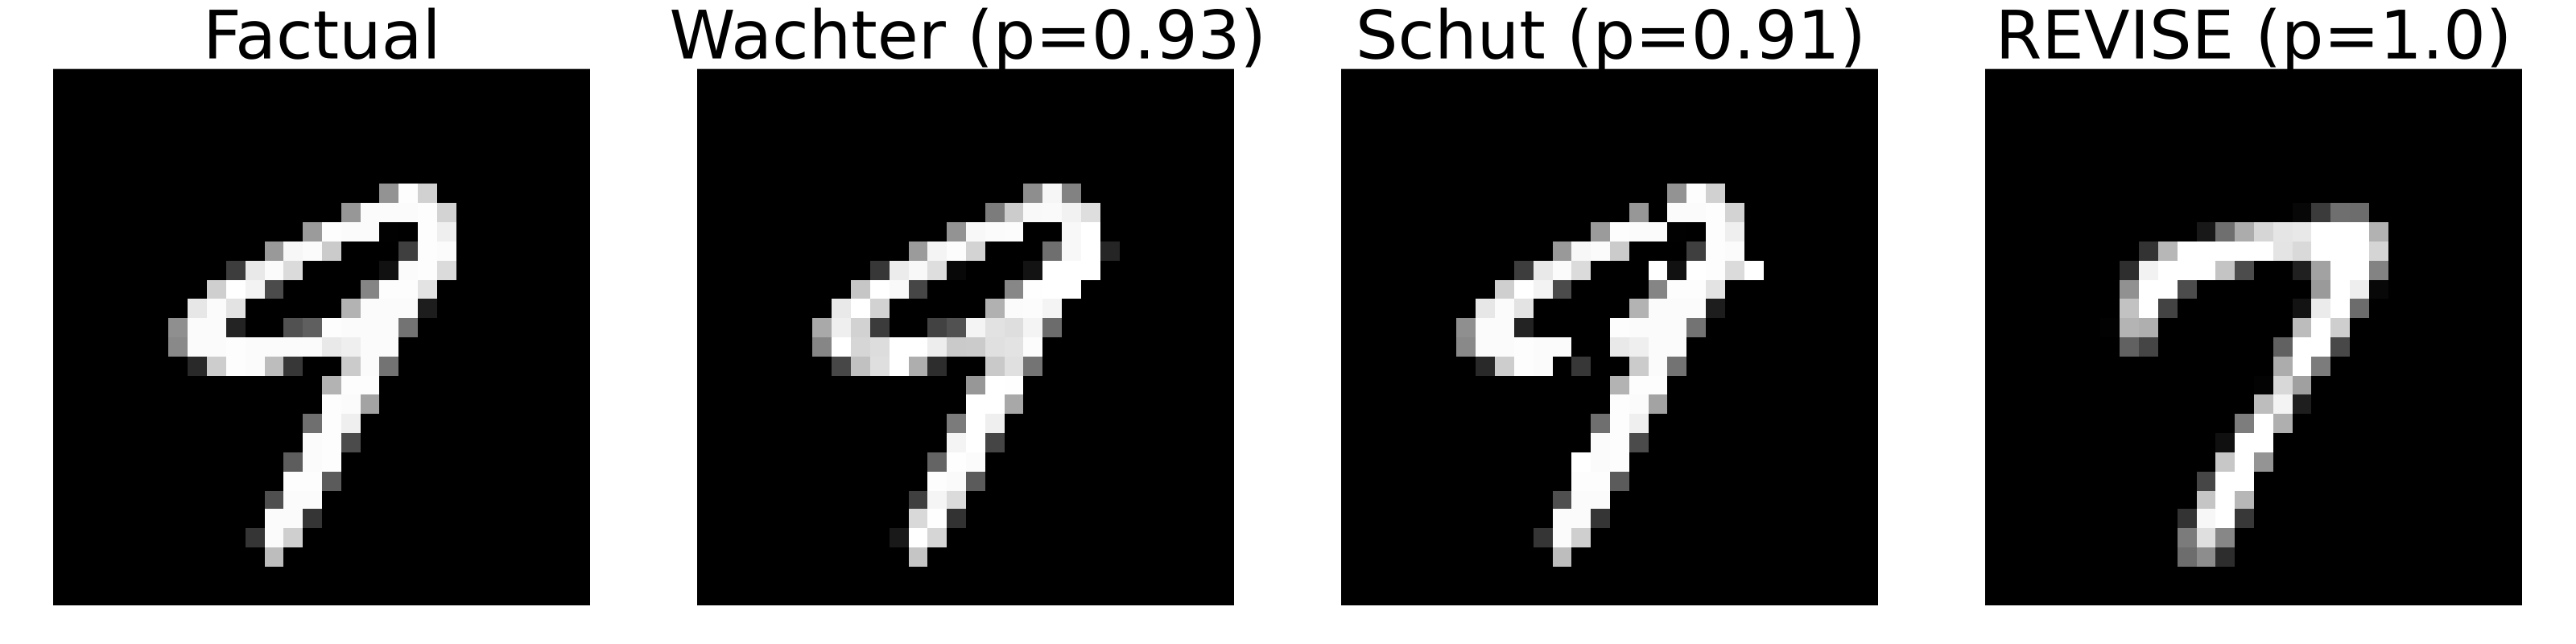
\includegraphics[width=0.4\textwidth]{../artifacts/results/images/mnist_motivation.png}
    \caption{Counterfactuals for turning a 9 (nine) into a 7 (seven): original image (left); then from left to right the counterfactuals generated using \textit{Wachter}, \textit{Schut} and \textit{REVISE}.}\label{fig:motiv}
  \end{figure}
  
  Since \textit{Wachter} is only concerned with proximity, the generated counterfactual is almost indistinguishable from the factual. The approach by~\citet{schut2021generating} expects a well-calibrated model that can generate predictive uncertainty estimates. Since this is not the case, the generated counterfactual looks like an adversarial example. Finally, the counterfactual generated by \textit{REVISE} looks much more plausible than the other two. But is it also more faithful to the behaviour of our \textit{MNIST} classifier? That is much less clear because the surrogate used by \textit{REVISE} introduces friction: the generated explanations no longer depend exclusively on the black-box model itself. 
  
  So which of the counterfactuals most faithfully explains the behaviour of our image classifier? Fidelity cannot help us to make that judgement, because all of these counterfactuals have full fidelity. Thus, fidelity is an insufficient evaluation metric to assess the faithfulness of CE. 
  
  \section{A New Notion of Faithfulness}\label{faithfulness}
  
  Considering the limitations of fidelity as demonstrated in the previous section, analogous to Definition~\ref{def:plausible}, we introduce a new notion of faithfulness in the context of CE:
  
  \begin{definition}[Faithful Counterfactuals]
    \label{def:faithful}
    Let $\mathcal{X}_{\theta}|\mathbf{y}^+ = p_{\theta}(\mathbf{x}|\mathbf{y}^+)$ denote the conditional distribution of $\mathbf{x}$ in the target class $\mathbf{y}^+$, where $\theta$ denotes the parameters of model $M_{\theta}$. Then for $\mathbf{x}^{\prime}$ to be considered a faithful counterfactual, we need: $\mathbf{x}^{\prime} \sim \mathcal{X}_{\theta}|\mathbf{y}^+$.
  \end{definition}
  
  In doing this, we merge in and nuance the concept of plausibility (Definition~\ref{def:plausible}) where the notion of `consistent with the data' becomes `consistent with what the model has learned about the data'.
  
  \subsection{Quantifying the Model's Generative Property}
  
  To assess counterfactuals with respect to Definition~\ref{def:faithful}, we need a way to quantify the posterior conditional distribution $p_{\theta}(\mathbf{x}|\mathbf{y}^+)$. To this end, we draw on recent advances in Energy-Based Modelling (EBM), a subdomain of machine learning that is concerned with generative or hybrid modelling~\citep{grathwohl2020your,du2020implicit}. In particular, note that if we fix $\mathbf{y}$ to our target value $\mathbf{y}^+$, we can conditionally draw from $p_{\theta}(\mathbf{x}|\mathbf{y}^+)$ by randomly initializing $\mathbf{x}_0$ and then using Stochastic Gradient Langevin Dynamics (SGLD) as follows, 
  
  \begin{equation}\label{eq:sgld}
    \begin{aligned}
      \mathbf{x}_{j+1} &\leftarrow \mathbf{x}_j - \frac{\epsilon^2}{2} \mathcal{E}(\mathbf{x}_j|\mathbf{y}^+) + \epsilon \mathbf{r}_j, && j=1,...,J
    \end{aligned}
  \end{equation}
  
  where $\mathbf{r}_j \sim \mathcal{N}(\mathbf{0},\mathbf{I})$ is the stochastic term and the step-size $\epsilon$ is typically polynomially decayed~\citep{welling2011bayesian}. The term $\mathcal{E}(\mathbf{x}_j|\mathbf{y}^+)$ denotes the model energy conditioned on the target class label $\mathbf{y}^+$ which we specify as the negative logit corresponding to the target class label $\mathbf{y}^*$. To allow for faster sampling, we follow the common practice of choosing the step-size $\epsilon$ and the standard deviation of $\mathbf{r}_j$ separately. While $\mathbf{x}_J$ is only guaranteed to distribute as $p_{\theta}(\mathbf{x}|\mathbf{y}^*)$ if $\epsilon \rightarrow 0$ and $J \rightarrow \infty$, the bias introduced for a small finite $\epsilon$ is negligible in practice \citep{murphy2023probabilistic,grathwohl2020your}. Appendix~\ref{app:jem} provides additional implementation details for any tasks related to energy-based modelling. 
  
  Generating multiple samples using SGLD thus yields an empirical distribution $\hat{\mathbf{X}}_{\theta,\mathbf{y}^+}$ that approximates what the model has learned about the input data. While in the context of EBM, this is usually done during training, we propose to repurpose this approach during inference in order to evaluate and generate faithful model explanations.
  
  \subsection{Evaluating Plausibility and Faithfulness}
  
  The parallels between our definitions of plausibility and faithfulness imply that we can also use similar evaluation metrics in both cases. Since existing work has focused heavily on plausibility, it offers a useful starting point. In particular,~\citet{guidotti2022counterfactual} have proposed an implausibility metric that measures the distance of the counterfactual from its nearest neighbour in the target class. As this distance is reduced, counterfactuals get more plausible under the assumption that the nearest neighbour itself is plausible in the sense of Definition~\ref{def:plausible}. In this work, we use the following adapted implausibility metric,
  
  \begin{equation}\label{eq:impl}
    \begin{aligned}
      \text{impl}(\mathbf{x}^{\prime},\mathbf{X}_{\mathbf{y}^+}) = \frac{1}{\lvert\mathbf{X}_{\mathbf{y}^+}\rvert} \sum_{\mathbf{x} \in \mathbf{X}_{\mathbf{y}^+}} \text{dist}(\mathbf{x}^{\prime},\mathbf{x})
    \end{aligned}
  \end{equation}
  
  where $\mathbf{x}^{\prime}$ denotes the counterfactual and $\mathbf{X}_{\mathbf{y}^+}$ is a subsample of the training data in the target class $\mathbf{y}^+$. By averaging over multiple samples in this manner, we avoid the risk that the nearest neighbour of $\mathbf{x}^{\prime}$ itself is not plausible according to Definition~\ref{def:plausible} (e.g an outlier).
  
  Equation~\ref{eq:impl} gives rise to a similar evaluation metric for unfaithfulness. We merely swap out the subsample of individuals in the target class for a subset $\hat{\mathbf{X}}^{n_E}_{\theta,\mathbf{y}^+}$ of the generated conditional samples:
  
  \begin{equation}\label{eq:faith}
    \begin{aligned}
      \text{unfaith}(\mathbf{x}^{\prime},\hat{\mathbf{X}}^{n_E}_{\theta,\mathbf{y}^+}) = \frac{1}{\lvert \hat{\mathbf{X}}^{n_E}_{\theta,\mathbf{y}^+}\rvert} \sum_{\mathbf{x} \in \hat{\mathbf{X}}^{n_E}_{\theta,\mathbf{y}^+}} \text{dist}(\mathbf{x}^{\prime},\mathbf{x})
    \end{aligned}
  \end{equation}
  
  Specifically, we form this subset based on the $n_E$ generated samples with the lowest energy. 
  
  \section{Energy-Constrained Conformal Counterfactuals}\label{meth}
  
  In this section, we describe \textit{ECCCo}, our proposed framework for generating Energy-Constrained Conformal Counterfactuals (ECCCos). It is based on the premise that counterfactuals should first and foremost be faithful. Plausibility, as a secondary concern, is then still attainable, but only to the degree that the black-box model itself has learned plausible explanations for the underlying data. 
  
  We begin by stating our proposed objective function, which involves tailored loss and penalty functions that we will explain in the following. In particular, we extend Equation~\ref{eq:general} as follows:
  
  \begin{equation} \label{eq:eccco}
    \begin{aligned}
    \mathbf{Z}^\prime= \arg \min_{\mathbf{Z}^\prime \in \mathcal{Z}^M}  &\{  {\text{yloss}(M_{\theta}(f(\mathbf{Z}^\prime)),\mathbf{y}^+)}+ \lambda_{1} {\text{dist}(f(\mathbf{Z}^\prime),\mathbf{x}) } \\
    &+ \lambda_2 \text{unfaith}(f(\mathbf{Z}^\prime),\hat{\mathbf{X}}^{n_E}_{\theta,\mathbf{y}^+}) + \lambda_3 \Omega(C_{\theta}(f(\mathbf{Z}^\prime);\alpha)) \} 
    \end{aligned} 
  \end{equation}
  
  The first penalty term involving $\lambda_1$ induces proximity like in~\citet{wachter2017counterfactual}. Our default choice for $\text{dist}(\cdot)$ is the L1 Norm due to its sparsity-inducing properties. The second penalty term involving $\lambda_2$ induces faithfulness by constraining the energy of the generated counterfactual where $\text{unfaith}(\cdot)$ corresponds to the metric defined in Equation~\ref{eq:faith}. The third and final penalty term involving $\lambda_3$ introduces a new concept: it ensures that the generated counterfactual is associated with low predictive uncertainty. As mentioned above,~\citet{schut2021generating} have shown that plausible counterfactuals can be generated implicitly through predictive uncertainty minimization. Unfortunately, this relies on the assumption that the model itself can provide predictive uncertainty estimates, which may be too restrictive in practice. 
  
  To relax this assumption, we leverage recent advances in Conformal Prediction (CP), an approach to predictive uncertainty quantification that has recently gained popularity~\citep{angelopoulos2021gentle,manokhin2022awesome}. Crucially for our intended application, CP is model-agnostic and can be applied during inference without placing any restrictions on model training. Intuitively, CP works under the premise of turning heuristic notions of uncertainty into rigorous uncertainty estimates by repeatedly sifting through the training data or a dedicated calibration dataset. Conformal classifiers produce prediction sets for individual inputs that include all output labels that can be reasonably attributed to the input. These sets tend to be larger for inputs that do not conform with the training data and are characterized by high predictive uncertainty. 
  
  In order to generate counterfactuals that are associated with low predictive uncertainty, we use a smooth set size penalty introduced by~\citet{stutz2022learning} in the context of conformal training:
  
  \begin{equation}\label{eq:setsize}
    \begin{aligned}
      \Omega(C_{\theta}(\mathbf{x};\alpha))&=\max \left(0, \sum_{\mathbf{y}\in\mathcal{Y}}C_{\theta,\mathbf{y}}(\mathbf{x}_i;\alpha) - \kappa \right)
    \end{aligned}
  \end{equation}
  
  Here, $\kappa \in \{0,1\}$ is a hyper-parameter and $C_{\theta,\mathbf{y}}(\mathbf{x}_i;\alpha)$ can be interpreted as the probability of label $\mathbf{y}$ being included in the prediction set. In order to compute this penalty for any black-box model we merely need to perform a single calibration pass through a holdout set $\mathcal{D}_{\text{cal}}$. Arguably, data is typically abundant and in most applications, practitioners tend to hold out a test data set anyway. Consequently, CP removes the restriction on the family of predictive models, at the small cost of reserving a subset of the available data for calibration. This particular case of conformal prediction is referred to as Split Conformal Prediction (SCP) as it involves splitting the training data into a proper training dataset and a calibration dataset. In addition to the smooth set size penalty, we have also experimented with the use of a tailored function for $\text{yloss}(\cdot)$ that enforces that only the target label $\mathbf{y}^+$ is included in the prediction set ~\citet{stutz2022learning}. Further details are provided in Appendix~\ref{app:cp}.
  
  \begin{figure}
    \centering
    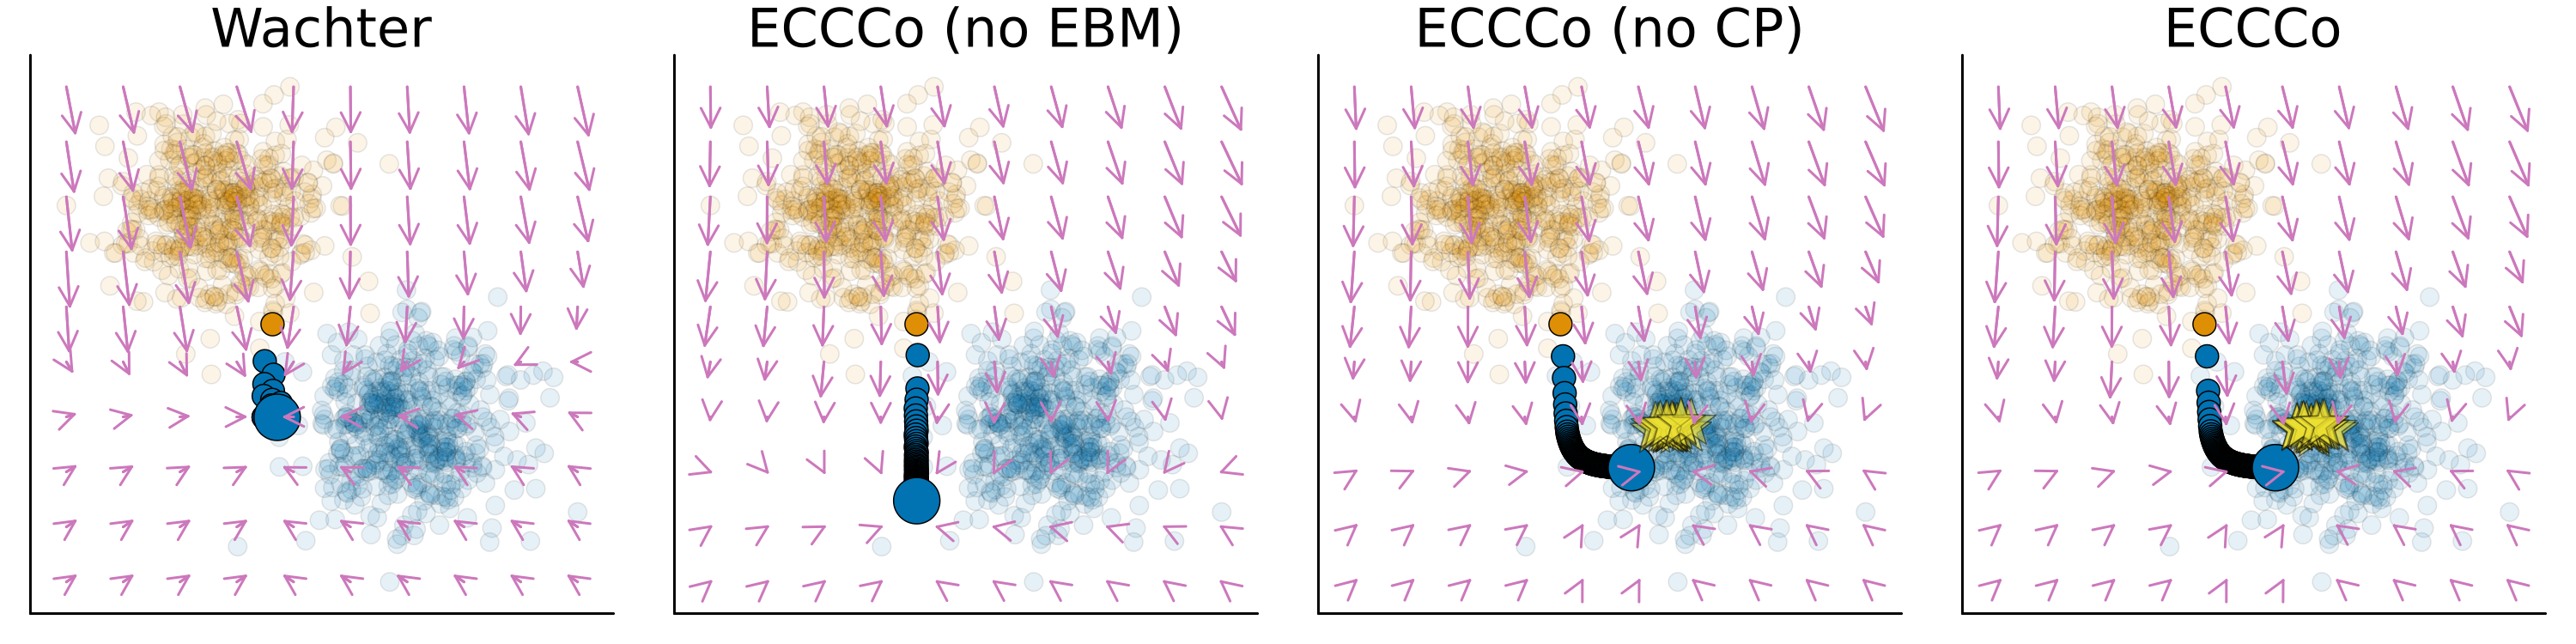
\includegraphics[width=0.5\textwidth]{../artifacts/results/images/poc_gradient_fields.png}
    \caption{Gradient fields and counterfactual paths for different generators. The objective is to generate a counterfual in the `blue' class for a sample from the `orange' class. Bright yellow stars indicate conditional samples generated through SGLD. The underlying classifier is a Joint Energy Model.}\label{fig:poc}
  \end{figure}
  
  \renewcommand{\algorithmicrequire}{\textbf{Input:}}
  \renewcommand{\algorithmicensure}{\textbf{Output:}}
  
  \begin{algorithm}
    \caption{The \textit{ECCCo} generator}\label{alg:eccco}
    \begin{algorithmic}[1]
      \Require $\mathbf{x}, \mathbf{y}^+, M_{\theta}, f, \Lambda=[\lambda_1,\lambda_2,\lambda_3], \alpha, \mathcal{D}, T, \eta, n_{\mathcal{B}}, n_E$ where $M_{\theta}(\mathbf{x})\neq\mathbf{y}^+$
      \Ensure $\mathbf{x}^\prime$
      \State Initialize $\mathbf{z}^\prime \gets f^{-1}(\mathbf{x})$ \Comment{Map to counterfactual state space.}
      \State Generate $\left\{\hat{\mathbf{x}}_{\theta,\mathbf{y}^+}\right\}_{n_{\mathcal{B}}} \gets p_{\theta}(\mathbf{x}_{\mathbf{y}^+})$ \Comment{Generate $n_{\mathcal{B}}$ samples using SGLD (Equation~\ref{eq:sgld}).}
      \State Store $\hat{\mathbf{X}}^{n_E}_{\theta,\mathbf{y}^+} \gets \left\{\hat{\mathbf{x}}_{\theta,\mathbf{y}^+}\right\}_{n_{\mathcal{B}}}$ \Comment{Choose $n_E$ lowest-energy samples.}
      \State Run \textit{SCP} for $M_{\theta}$ using $\mathcal{D}$ \Comment{Calibrate model through Split Conformal Prediction.}
      \State Initialize $t \gets 0$
      \While{\textit{not converged} or $t < T$} \Comment{For convergence conditions see Appendix~\ref{app:eccco}.}
      \State $\mathbf{z}^\prime \gets \mathbf{z}^\prime - \eta \nabla_{\mathbf{z}^\prime} \mathcal{L}(\mathbf{z}^\prime,\mathbf{y}^+,\hat{\mathbf{X}}^{n_E}_{\theta,\mathbf{y}^+}; \Lambda, \alpha)$ \Comment{Take gradient step of size $\eta$.}
      \State $t \gets t+1$
      \EndWhile
      \State $\mathbf{x}^\prime \gets f(\mathbf{z}^\prime)$ \Comment{Map back to feature space.}
    \end{algorithmic}
  \end{algorithm}
  
  To provide some further intuition about our objective defined in Equation~\ref{eq:eccco}, Figure~\ref{fig:poc} illustrates how the different components affect the counterfactual search for a synthetic dataset. The underlying classifier is a Joint Energy Model (\textit{JEM}) that was trained to predict the output class (`blue' or `orange') and generate class-conditional samples~\citep{grathwohl2020your}. We have used four different generator flavours to produce a counterfactual in the `blue' class for a sample from the `orange' class: \textit{Wachter}, which only uses the first penalty ($\lambda_2=\lambda_3=0$); \textit{ECCCo (no EBM)}, which does not constrain energy ($\lambda_2=0$); \textit{ECCCo (no CP)}, which involves no set size penalty ($\lambda_3=0$); and, finally, \textit{ECCCo}, which involves all penalties defined in Equation~\ref{eq:eccco}. Arrows indicate (negative) gradients with respect to the objective function at different points in the feature space. 
  
  While \textit{Wachter} generates a valid counterfactual, it ends up close to the original starting point consistent with its objective. \textit{ECCCo (no EBM)} pushes the counterfactual further into the target domain to minimize predictive uncertainty, but the outcome is still not plausible. The counterfactual produced by \textit{ECCCo (no CP)} is attracted by the generated samples shown in bright yellow. Since the \textit{JEM} has learned the conditional input distribution reasonably well in this case, the counterfactuals are both faithful and plausible. Finally, the outcome for \textit{ECCCo} looks similar, but the additional smooth set size penalty leads to somewhat faster convergence. 
  
  Algorithm~\ref{alg:eccco} describes how exactly \textit{ECCCo} works. For the sake of simplicity and without loss of generality, we limit our attention to generating a single counterfactual $\mathbf{x}^\prime=f(\mathbf{z}^\prime)$. The counterfactual state $\mathbf{z}^\prime$ is initialized by passing the factual $\mathbf{x}$ through a simple feature transformer $f^{-1}$. Next, we generate $n_{\mathcal{B}}$ conditional samples $\hat{\mathbf{x}}_{\theta,\mathbf{y}^+}$ using SGLD (Equation~\ref{eq:sgld}) and store the $n_E$ instances with the lowest energy. We then calibrate the model $M_{\theta}$ through Split Conformal Prediction. Finally, we search counterfactuals through gradient descent where $\mathcal{L}(\mathbf{z}^\prime,\mathbf{y}^+,\hat{\mathbf{X}}^{n_E}_{\theta,\mathbf{y}^+}; \Lambda, \alpha)$ denotes our loss function defined in Equation~\ref{eq:eccco}. The search terminates once the convergence criterium is met or the maximum number of iterations $T$ has been exhausted. Note that the choice of convergence criterium has important implications on the final counterfactual which we explain in Appendix~\ref{app:eccco}.
  
  \section{Empirical Analysis}\label{emp}
  
  Our goal in this section is to shed light on the following research questions:
  
  \begin{question}[Faithfulness]\label{rq:faithfulness}
    Are ECCCos more faithful than counterfactuals produced by our benchmark generators?
  \end{question}
  
  \begin{question}[Balancing Objectives]\label{rq:plausibility}
    Compared to our benchmark generators, how do ECCCos balance the two key objectives of faithfulness and plausibility?
  \end{question}
  
  The second question is motivated by the intuition that faithfulness and plausibility should coincide for models that have learned plausible explanations of the data. Next, we first briefly describe our experimental setup before presenting our main results.
  
  \subsection{Experimental Setup}
  
  To assess and benchmark the performance of our proposed generator against the state of the art, we generate multiple counterfactuals for different models and datasets. In particular, we compare \textit{ECCCo} and its variants to the following counterfactual generators that were introduced above: firstly; \textit{Schut}, which works under the premise of minimizing predictive uncertainty; secondly, \textit{REVISE}, which is state-of-the-art with respect to plausibility; and, finally, \textit{Wachter}, which serves as our baseline. 
  
  We use both synthetic and real-world datasets from different domains, all of which are publicly available and commonly used to train and benchmark classification algorithms. We synthetically generate a dataset containing two \textit{Linearly Separable} Gaussian clusters ($n=1000$), as well as the well-known \textit{Circles} ($n=1000$) and \textit{Moons} ($n=2500$) data. Since these data are generated by distributions of varying degrees of complexity, they allow us to assess how the generators and our proposed evaluation metrics handle this.
  
  As for real-world data, we follow~\citet{schut2021generating} and use the \textit{MNIST}~\citep{lecun1998mnist} dataset containing images of handwritten digits such as the example shown above in Figure~\ref{fig:motiv}. From the social sciences domain, we include Give Me Some Credit (\textit{GMSC})~\citep{kaggle2011give}: a tabular dataset that has been studied extensively in the literature on Algorithmic Recourse~\citep{pawelczyk2021carla}. It consists of 11 numeric features that can be used to predict the binary outcome variable indicating whether retail borrowers experience financial distress. 
  
  For the predictive modelling tasks, we use simple neural networks (\textit{MLP}) and Joint Energy Models (\textit{JEM}). For the more complex real-world datasets we also use ensembling in each case. Both joint-energy modelling and ensembling have been associated with improved generative properties and adversarial robustness~\citep{grathwohl2020your,lakshminarayanan2016simple}, so we expect this to be positively correlated with the plausibility of ECCCos. To account for stochasticity, we generate multiple counterfactuals for each target class, generator, model and dataset. Specifically, we randomly sample $n^{-}$ times from the subset of individuals for which the given model predicts the non-target class $\mathbf{y}^{-}$ given the current target. We set $n^{-}=25$ for all of our synthetic datasets, $n^{-}=10$ for \textit{GMSC} and $n^{-}=5$ for \textit{MNIST}. Full details concerning our parameter choices, training procedures and model performance can be found in Appendix~\ref{app:setup}.
  
  \subsection{Results for Synthetic Data}
  
  Table~\ref{tab:results-synthetic} shows the key results for the synthetic datasets separated by model (first column) and generator (second column). The numerical columns show sample averages and standard deviations of our key evaluation metrics computed across all counterfactuals. We have highlighted the best outcome for each model and metric in bold. To provide some sense of effect sizes, we have added asterisks to indicate that a given value is at least one ($*$) or two ($**$) standard deviations lower than the baseline (\textit{Wachter}).
  
  Starting with the high-level results for our \textit{Linearly Separable} data, we find that \textit{ECCCo} produces the most faithful counterfactuals for both black-box models. This is consistent with our design since \textit{ECCCo} directly enforces faithfulness through regularization. Crucially though, \textit{ECCCo} also produces the most plausible counterfactuals for both models. This dataset is so simple that even the \textit{MLP} has learned plausible explanations of the input data. Zooming in on the granular details for the \textit{Linearly Separable} data, the results for \textit{ECCCo (no CP)} and \textit{ECCCo (no EBM)} indicate that the positive results are dominated by the effect of quantifying and leveraging the model's generative property (EBM). Conformal Prediction alone only leads to marginally improved faithfulness and plausibility.
  
  The findings for the \textit{Moons} dataset are broadly in line with the findings so far: for the \textit{JEM}, \textit{ECCCo} yields substantially more faithful and plausible counterfactuals than all other generators. For the \textit{MLP}, faithfulness is maintained but counterfactuals are not plausible. This high-level pattern is broadly consistent with other more complex datasets and supportive of our narrative, so it is worth highlighting: ECCCos consistently achieve high faithfulness, which---subject to the quality of the model itself---coincides with high plausibility. By comparison, \textit{REVISE} yields the most plausible counterfactuals for the \textit{MLP}, but it does so at the cost of faithfulness. We also observe that the best results for \textit{ECCCo} are achieved when using both penalties. Once again though, the generative component (EBM) has a stronger impact on the positive results for the \textit{JEM}.
  
  For the \textit{Circles} data, it appears that \textit{REVISE} performs well, but we note that it generates valid counterfactuals only half of the time (see Appendix~\ref{app:results} for a complete overview including additional common evaluation metrics). The underlying VAE with default parameters has not adequately learned the data-generating process. Of course, it is possible to improve generative performance through hyperparameter tuning but this example serves to illustrate that \textit{REVISE} depends on the quality of its surrogate. Independent of the outcome for \textit{REVISE}, however, the results do not seem to indicate that \textit{ECCCo} substantially improves faithfulness and plausibility for the \textit{Circles} data. We think this points to a limitation of our evaluation metrics rather than \textit{ECCCo} itself: computing average distances fails to account for the `wraparound' effect associated with circular data~\citep{gill2010circular}.
  
  \import{contents/}{table-synthetic.tex}
  
  \subsection{Results for Real-World Data}
  
  The results for our real-world datasets are shown in Table~\ref{tab:results-real-world}. Once again the findings indicate that the plausibility of ECCCos is positively correlated with the capacity of the black-box model to distinguish plausible from implausible inputs. The case is very clear for \textit{MNIST}: ECCCos are consistently more faithful than the counterfactuals produced by our benchmark generators and their plausibility gradually improves through ensembling and joint-energy modelling. Interestingly, faithfulness also gradually improves for \textit{REVISE}. This indicates that as our models improve, their generative capacity approaches that of the surrogate VAE used by \textit{REVISE}. The VAE still outperforms our classifiers in this regard, as evident from the fact that \textit{ECCCo} never quite reaches the same level of plausibility as \textit{REVISE}. With reference to Appendix~\ref{app:results} we note that the results for \textit{Schut} need to be discounted as it rarely produces valid counterfactuals for \textit{MNIST}. Relatedly, we find that \textit{ECCCo} is the only generator that consistently achieves full validity. Finally, it is worth noting that \textit{ECCCo} produces counterfactual images with the lowest average predictive uncertainty for all models. 
  
  For the tabular credit dataset (\textit{GMSC}) it is inherently challenging to use deep neural networks in order to achieve good discriminative performance~\citep{borisov2021deep,grinsztajn2022why} and generative performance~\citep{liu2023goggle}, respectively. In order to achieve high plausibility, \textit{ECCCo} effectively requires classifiers to achieve good performance for both tasks. Since this is a challenging task even for Joint Energy Models, it is not surprising to find that even though \textit{ECCCo} once again achieves state-of-the-art faithfulness, it is outperformed by \textit{REVISE} and \textit{Schut} with respect to plausibility.
  
  \subsection{Key Takeways}
  
  To conclude this section, we summarize our findings with reference to the opening questions. The results clearly demonstrate that \textit{ECCCo} consistently achieves state-of-the-art faithfulness, as it was designed to do (Research Question~\ref{rq:faithfulness}). A related important finding is that \textit{ECCCo} yields highly plausible explanations provided that they faithfully describe model behaviour (Research Question~\ref{rq:plausibility}). \textit{ECCCo} achieves this result primarily by leveraging the model's generative property.
  
  \import{contents/}{table-real-world.tex}
  
  \section{Limitations}
  
  Even though we have taken considerable measures to study our proposed methodology carefully, limitations can still be identified. In particular, we have found that the performance of \textit{ECCCo} is sensitive to hyperparameter choices. In order to achieve faithfulness, we generally had to penalise the distance from generated samples slightly more than the distance from factual values.
  
  Conversely, we have not found that strongly penalising prediction set sizes had any discernable effect. Our results indicate that CP alone is often not sufficient to achieve faithfulness and plausibility, although we acknowledge that this needs to be investigated more thoroughly through future work.
  
  While our approach is readily applicable to models with gradient access like deep neural networks, more work is needed to generalise it to other machine learning models such as decision trees. Relatedly, common challenges associated with Energy-Based Modelling including sensitivity to scale, training instabilities and sensitivity to hyperparameters also apply to \textit{ECCCo}.
  
  \section{Conclusion}
  
  This work leverages recent advances in Energy-Based Modelling and Conformal Prediction in the context of Explainable Artificial Intelligence. We have proposed a new way to generate counterfactuals that are maximally faithful to the black-box model they aim to explain. Our proposed generator, \textit{ECCCo}, produces plausible counterfactuals if and only if the black-box model itself has learned realistic explanations for the data, which we have demonstrated through rigorous empirical analysis. This should enable researchers and practitioners to use counterfactuals in order to discern trustworthy models from unreliable ones. While the scope of this work limits its generalizability, we believe that \textit{ECCCo} offers a solid baseline for future work on faithful Counterfactual Explanations.
  
  \section{Acknowledgments}
  
  Some of the members of TU Delft were partially funded by ICAI AI for Fintech Research, an ING — TU Delft
  collaboration.
  
  \bibliography{bib}

\end{document}
